% Options for packages loaded elsewhere
\PassOptionsToPackage{unicode}{hyperref}
\PassOptionsToPackage{hyphens}{url}
%
\documentclass[
]{article}
\usepackage{lmodern}
\usepackage{amssymb,amsmath}
\usepackage{ifxetex,ifluatex}
\ifnum 0\ifxetex 1\fi\ifluatex 1\fi=0 % if pdftex
  \usepackage[T1]{fontenc}
  \usepackage[utf8]{inputenc}
  \usepackage{textcomp} % provide euro and other symbols
\else % if luatex or xetex
  \usepackage{unicode-math}
  \defaultfontfeatures{Scale=MatchLowercase}
  \defaultfontfeatures[\rmfamily]{Ligatures=TeX,Scale=1}
\fi
% Use upquote if available, for straight quotes in verbatim environments
\IfFileExists{upquote.sty}{\usepackage{upquote}}{}
\IfFileExists{microtype.sty}{% use microtype if available
  \usepackage[]{microtype}
  \UseMicrotypeSet[protrusion]{basicmath} % disable protrusion for tt fonts
}{}
\makeatletter
\@ifundefined{KOMAClassName}{% if non-KOMA class
  \IfFileExists{parskip.sty}{%
    \usepackage{parskip}
  }{% else
    \setlength{\parindent}{0pt}
    \setlength{\parskip}{6pt plus 2pt minus 1pt}}
}{% if KOMA class
  \KOMAoptions{parskip=half}}
\makeatother
\usepackage{xcolor}
\IfFileExists{xurl.sty}{\usepackage{xurl}}{} % add URL line breaks if available
\IfFileExists{bookmark.sty}{\usepackage{bookmark}}{\usepackage{hyperref}}
\hypersetup{
  pdftitle={Taller 2: Análisis ANOVA-MANOVA},
  pdfauthor={JRojas, MRamirez, LRomero},
  hidelinks,
  pdfcreator={LaTeX via pandoc}}
\urlstyle{same} % disable monospaced font for URLs
\usepackage[margin=1in]{geometry}
\usepackage{color}
\usepackage{fancyvrb}
\newcommand{\VerbBar}{|}
\newcommand{\VERB}{\Verb[commandchars=\\\{\}]}
\DefineVerbatimEnvironment{Highlighting}{Verbatim}{commandchars=\\\{\}}
% Add ',fontsize=\small' for more characters per line
\usepackage{framed}
\definecolor{shadecolor}{RGB}{248,248,248}
\newenvironment{Shaded}{\begin{snugshade}}{\end{snugshade}}
\newcommand{\AlertTok}[1]{\textcolor[rgb]{0.94,0.16,0.16}{#1}}
\newcommand{\AnnotationTok}[1]{\textcolor[rgb]{0.56,0.35,0.01}{\textbf{\textit{#1}}}}
\newcommand{\AttributeTok}[1]{\textcolor[rgb]{0.77,0.63,0.00}{#1}}
\newcommand{\BaseNTok}[1]{\textcolor[rgb]{0.00,0.00,0.81}{#1}}
\newcommand{\BuiltInTok}[1]{#1}
\newcommand{\CharTok}[1]{\textcolor[rgb]{0.31,0.60,0.02}{#1}}
\newcommand{\CommentTok}[1]{\textcolor[rgb]{0.56,0.35,0.01}{\textit{#1}}}
\newcommand{\CommentVarTok}[1]{\textcolor[rgb]{0.56,0.35,0.01}{\textbf{\textit{#1}}}}
\newcommand{\ConstantTok}[1]{\textcolor[rgb]{0.00,0.00,0.00}{#1}}
\newcommand{\ControlFlowTok}[1]{\textcolor[rgb]{0.13,0.29,0.53}{\textbf{#1}}}
\newcommand{\DataTypeTok}[1]{\textcolor[rgb]{0.13,0.29,0.53}{#1}}
\newcommand{\DecValTok}[1]{\textcolor[rgb]{0.00,0.00,0.81}{#1}}
\newcommand{\DocumentationTok}[1]{\textcolor[rgb]{0.56,0.35,0.01}{\textbf{\textit{#1}}}}
\newcommand{\ErrorTok}[1]{\textcolor[rgb]{0.64,0.00,0.00}{\textbf{#1}}}
\newcommand{\ExtensionTok}[1]{#1}
\newcommand{\FloatTok}[1]{\textcolor[rgb]{0.00,0.00,0.81}{#1}}
\newcommand{\FunctionTok}[1]{\textcolor[rgb]{0.00,0.00,0.00}{#1}}
\newcommand{\ImportTok}[1]{#1}
\newcommand{\InformationTok}[1]{\textcolor[rgb]{0.56,0.35,0.01}{\textbf{\textit{#1}}}}
\newcommand{\KeywordTok}[1]{\textcolor[rgb]{0.13,0.29,0.53}{\textbf{#1}}}
\newcommand{\NormalTok}[1]{#1}
\newcommand{\OperatorTok}[1]{\textcolor[rgb]{0.81,0.36,0.00}{\textbf{#1}}}
\newcommand{\OtherTok}[1]{\textcolor[rgb]{0.56,0.35,0.01}{#1}}
\newcommand{\PreprocessorTok}[1]{\textcolor[rgb]{0.56,0.35,0.01}{\textit{#1}}}
\newcommand{\RegionMarkerTok}[1]{#1}
\newcommand{\SpecialCharTok}[1]{\textcolor[rgb]{0.00,0.00,0.00}{#1}}
\newcommand{\SpecialStringTok}[1]{\textcolor[rgb]{0.31,0.60,0.02}{#1}}
\newcommand{\StringTok}[1]{\textcolor[rgb]{0.31,0.60,0.02}{#1}}
\newcommand{\VariableTok}[1]{\textcolor[rgb]{0.00,0.00,0.00}{#1}}
\newcommand{\VerbatimStringTok}[1]{\textcolor[rgb]{0.31,0.60,0.02}{#1}}
\newcommand{\WarningTok}[1]{\textcolor[rgb]{0.56,0.35,0.01}{\textbf{\textit{#1}}}}
\usepackage{longtable,booktabs}
% Correct order of tables after \paragraph or \subparagraph
\usepackage{etoolbox}
\makeatletter
\patchcmd\longtable{\par}{\if@noskipsec\mbox{}\fi\par}{}{}
\makeatother
% Allow footnotes in longtable head/foot
\IfFileExists{footnotehyper.sty}{\usepackage{footnotehyper}}{\usepackage{footnote}}
\makesavenoteenv{longtable}
\usepackage{graphicx,grffile}
\makeatletter
\def\maxwidth{\ifdim\Gin@nat@width>\linewidth\linewidth\else\Gin@nat@width\fi}
\def\maxheight{\ifdim\Gin@nat@height>\textheight\textheight\else\Gin@nat@height\fi}
\makeatother
% Scale images if necessary, so that they will not overflow the page
% margins by default, and it is still possible to overwrite the defaults
% using explicit options in \includegraphics[width, height, ...]{}
\setkeys{Gin}{width=\maxwidth,height=\maxheight,keepaspectratio}
% Set default figure placement to htbp
\makeatletter
\def\fps@figure{htbp}
\makeatother
\setlength{\emergencystretch}{3em} % prevent overfull lines
\providecommand{\tightlist}{%
  \setlength{\itemsep}{0pt}\setlength{\parskip}{0pt}}
\setcounter{secnumdepth}{-\maxdimen} % remove section numbering

\title{Taller 2: Análisis ANOVA-MANOVA}
\author{JRojas, MRamirez, LRomero}
\date{6/24/2020}

\begin{document}
\maketitle

\hypertarget{introducciuxf3n}{%
\section{Introducción}\label{introducciuxf3n}}

A continuación se presentan una serie de ejercicios propuesto que
permitiran interiorizar el análisis de datos multivariados utilizandos
las técnicas ANOVA y MANOVA. Estos ejercicios hacen parte del contenido
académico desarrollado por el profesor Aquiles Enrique Darghan Contreras
referente a la asignatura de Métodos Multivariados.

Previo a la solución de los ejercicios es necesario instalar y cargar
las siguientes librerías.

\begin{Shaded}
\begin{Highlighting}[]
\KeywordTok{library}\NormalTok{(readxl)}
\end{Highlighting}
\end{Shaded}

\begin{verbatim}
## Warning: package 'readxl' was built under R version 3.6.3
\end{verbatim}

\begin{Shaded}
\begin{Highlighting}[]
\KeywordTok{library}\NormalTok{(ggplot2)}
\end{Highlighting}
\end{Shaded}

\begin{verbatim}
## Warning: package 'ggplot2' was built under R version 3.6.3
\end{verbatim}

\begin{Shaded}
\begin{Highlighting}[]
\KeywordTok{library}\NormalTok{(mvShapiroTest)}
\KeywordTok{library}\NormalTok{(biotools)}
\end{Highlighting}
\end{Shaded}

\begin{verbatim}
## Warning: package 'biotools' was built under R version 3.6.3
\end{verbatim}

\begin{verbatim}
## Warning: package 'rpanel' was built under R version 3.6.3
\end{verbatim}

\begin{verbatim}
## Warning: package 'SpatialEpi' was built under R version 3.6.3
\end{verbatim}

\begin{verbatim}
## Warning: package 'sp' was built under R version 3.6.3
\end{verbatim}

\begin{verbatim}
## ---
## biotools version 3.1
\end{verbatim}

\begin{Shaded}
\begin{Highlighting}[]
\KeywordTok{library}\NormalTok{(outliers)}
\end{Highlighting}
\end{Shaded}

\hypertarget{datos}{%
\subsection{Datos}\label{datos}}

Los ejercicios mostrados son desarrollados a partir de los siguientes
datos correspondientes a una toma realizada con un espectroradiometro en
los anchos de bandas correspondientes a 560 \emph{nm} y 720 \emph{nm} de
las especies \emph{SS}, \emph{JL} y \emph{LP}

\begin{longtable}[]{@{}lll@{}}
\toprule
D\_560nm & D\_720nm & Species\tabularnewline
\midrule
\endhead
9.33 & 19.14 & SS\tabularnewline
8.74 & 19.55 & SS\tabularnewline
9.31 & 19.24 & SS\tabularnewline
8.27 & 16.37 & SS\tabularnewline
10.22 & 25 & SS\tabularnewline
10.13 & 25.32 & SS\tabularnewline
10.42 & 27.12 & SS\tabularnewline
10.62 & 26.28 & SS\tabularnewline
15.25 & 38.89 & SS\tabularnewline
16.22 & 36.67 & SS\tabularnewline
17.24 & 40.74 & SS\tabularnewline
12.77 & 67.5 & SS\tabularnewline
12.07 & 33.03 & JL\tabularnewline
11.03 & 32.37 & JL\tabularnewline
12.48 & 31.31 & JL\tabularnewline
12.12 & 33.33 & JL\tabularnewline
15.38 & 40 & JL\tabularnewline
14.21 & 40.48 & JL\tabularnewline
9.69 & 33.9 & JL\tabularnewline
14.35 & 40.15 & JL\tabularnewline
38.71 & 77.14 & JL\tabularnewline
44.74 & 78.57 & JL\tabularnewline
36.67 & 71.43 & JL\tabularnewline
37.21 & 45 & JL\tabularnewline
8.73 & 23.27 & LP\tabularnewline
7.94 & 20.87 & LP\tabularnewline
8.37 & 22.16 & LP\tabularnewline
7.86 & 21.78 & LP\tabularnewline
8.45 & 26.32 & LP\tabularnewline
6.79 & 22.73 & LP\tabularnewline
8.34 & 26.67 & LP\tabularnewline
7.54 & 24.87 & LP\tabularnewline
14.04 & 44.44 & LP\tabularnewline
13.51 & 37.93 & LP\tabularnewline
13.33 & 37.93 & LP\tabularnewline
12.77 & 60.87 & LP\tabularnewline
\bottomrule
\end{longtable}

Los datos se encuentran disponibles en un archivo de
\href{https://docs.google.com/spreadsheets/d/1KeSKTZRl8or_yGPC7_876nhyAQlxqjK3EC9UVl8n4yc/edit?usp=sharing}{google
sheets} para quien desee realizar los mismos ejercicios presentados.

Como primer paso los datos son cargados a la variable denominada
\emph{Reflectancia}

\begin{Shaded}
\begin{Highlighting}[]
\NormalTok{Reflectancia <-}\StringTok{ }\KeywordTok{read_excel}\NormalTok{(}\StringTok{"Datos_ANOVA_MANOVA.xlsx"}\NormalTok{)}
\end{Highlighting}
\end{Shaded}

\hypertarget{punto-1-manova}{%
\section{Punto 1: MANOVA}\label{punto-1-manova}}

Para el análisis se realizan las gráficas para cada longitud de onda y
un gráfico de dispersión que muestre la relación de las dos:

\begin{Shaded}
\begin{Highlighting}[]
\KeywordTok{ggplot}\NormalTok{(}\DataTypeTok{data=}\NormalTok{Reflectancia, }\KeywordTok{aes}\NormalTok{(Species,D_560nm)) }\OperatorTok{+}\StringTok{ }\KeywordTok{geom_point}\NormalTok{() }\OperatorTok{+}\StringTok{ }\KeywordTok{ggtitle}\NormalTok{(}\StringTok{"Comportamiento Firma 560 nm"}\NormalTok{) }\OperatorTok{+}\StringTok{ }\KeywordTok{xlab}\NormalTok{(}\StringTok{"Especies"}\NormalTok{) }\OperatorTok{+}\StringTok{ }\KeywordTok{ylab}\NormalTok{(}\StringTok{"Reflectancia"}\NormalTok{)}
\end{Highlighting}
\end{Shaded}

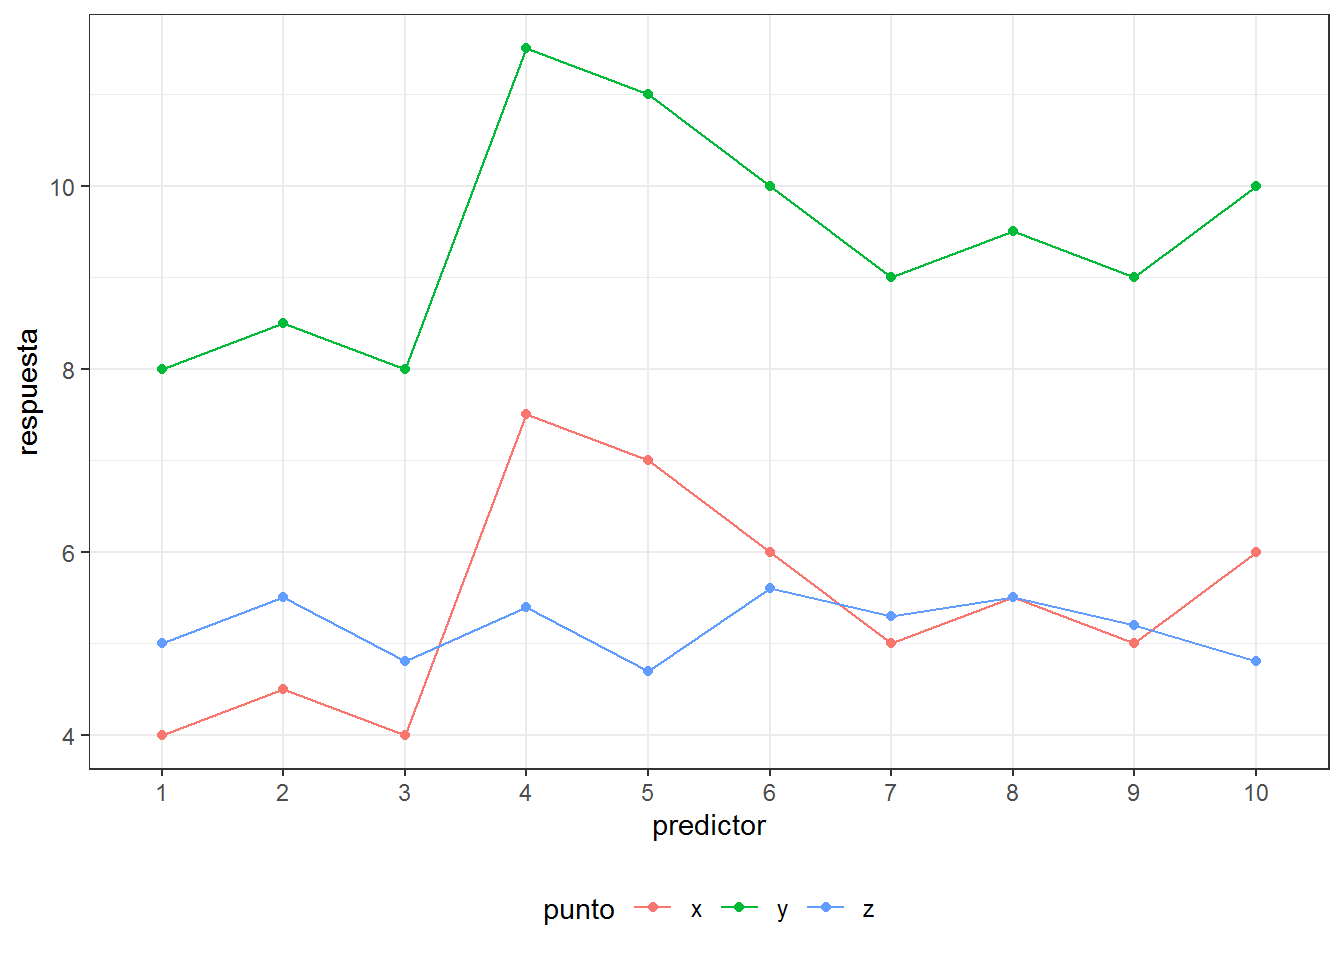
\includegraphics{Taller3_files/figure-latex/unnamed-chunk-3-1.pdf}

\begin{Shaded}
\begin{Highlighting}[]
\KeywordTok{ggplot}\NormalTok{(}\DataTypeTok{data=}\NormalTok{Reflectancia, }\KeywordTok{aes}\NormalTok{(Species,D_720nm)) }\OperatorTok{+}\StringTok{ }\KeywordTok{geom_point}\NormalTok{() }\OperatorTok{+}\StringTok{ }\KeywordTok{ggtitle}\NormalTok{(}\StringTok{"Comportamiento Firma 720 nm"}\NormalTok{) }\OperatorTok{+}\StringTok{ }\KeywordTok{xlab}\NormalTok{(}\StringTok{"Especies"}\NormalTok{) }\OperatorTok{+}\StringTok{ }\KeywordTok{ylab}\NormalTok{(}\StringTok{"Reflectancia"}\NormalTok{)}
\end{Highlighting}
\end{Shaded}

\includegraphics{Taller3_files/figure-latex/unnamed-chunk-3-2.pdf}

\begin{Shaded}
\begin{Highlighting}[]
\KeywordTok{ggplot}\NormalTok{(}\DataTypeTok{data=}\NormalTok{Reflectancia, }\KeywordTok{aes}\NormalTok{(D_560nm,D_720nm, }\DataTypeTok{color=}\NormalTok{Species)) }\OperatorTok{+}\StringTok{ }\KeywordTok{geom_point}\NormalTok{() }\OperatorTok{+}\StringTok{ }\KeywordTok{ggtitle}\NormalTok{(}\StringTok{"Comportamiento Firma 560 nm vs 720 nm"}\NormalTok{)}
\end{Highlighting}
\end{Shaded}

\includegraphics{Taller3_files/figure-latex/unnamed-chunk-3-3.pdf}

Se procede a realizar el análisis MANOVA y se presenta un resumen del
mismo con la hipotesis con el test de \emph{Wilks}

\begin{Shaded}
\begin{Highlighting}[]
\NormalTok{MN=}\KeywordTok{manova}\NormalTok{(}\KeywordTok{cbind}\NormalTok{(Reflectancia}\OperatorTok{$}\NormalTok{D_560nm,Reflectancia}\OperatorTok{$}\NormalTok{D_720nm) }\OperatorTok{~}\StringTok{ }\NormalTok{Reflectancia}\OperatorTok{$}\NormalTok{Species)}
\NormalTok{MN}
\end{Highlighting}
\end{Shaded}

\begin{verbatim}
## Call:
##    manova(cbind(Reflectancia$D_560nm, Reflectancia$D_720nm) ~ Reflectancia$Species)
## 
## Terms:
##                 Reflectancia$Species Residuals
## resp 1                       965.181  2147.714
## resp 2                      2026.856  7536.997
## Deg. of Freedom                    2        33
## 
## Residual standard errors: 8.067357 15.11271
## Estimated effects may be unbalanced
\end{verbatim}

\begin{Shaded}
\begin{Highlighting}[]
\KeywordTok{summary}\NormalTok{(MN,}\DataTypeTok{test=}\StringTok{"Wilks"}\NormalTok{)}
\end{Highlighting}
\end{Shaded}

\begin{verbatim}
##                      Df   Wilks approx F num Df den Df Pr(>F)  
## Reflectancia$Species  2 0.67704   3.4452      4     64  0.013 *
## Residuals            33                                        
## ---
## Signif. codes:  0 '***' 0.001 '**' 0.01 '*' 0.05 '.' 0.1 ' ' 1
\end{verbatim}

Observandose que se presentan diferencias significativas entre las dos
especies

\hypertarget{punto-2-anova}{%
\section{Punto 2: ANOVA}\label{punto-2-anova}}

\begin{Shaded}
\begin{Highlighting}[]
\NormalTok{AV1=}\KeywordTok{aov}\NormalTok{(Reflectancia}\OperatorTok{$}\NormalTok{D_560nm }\OperatorTok{~}\StringTok{ }\NormalTok{Reflectancia}\OperatorTok{$}\NormalTok{Species)}
\KeywordTok{summary}\NormalTok{(AV1)}
\end{Highlighting}
\end{Shaded}

\begin{verbatim}
##                      Df Sum Sq Mean Sq F value  Pr(>F)   
## Reflectancia$Species  2  965.2   482.6   7.415 0.00219 **
## Residuals            33 2147.7    65.1                   
## ---
## Signif. codes:  0 '***' 0.001 '**' 0.01 '*' 0.05 '.' 0.1 ' ' 1
\end{verbatim}

\begin{Shaded}
\begin{Highlighting}[]
\NormalTok{AV2=}\KeywordTok{aov}\NormalTok{(Reflectancia}\OperatorTok{$}\NormalTok{D_720nm }\OperatorTok{~}\StringTok{ }\NormalTok{Reflectancia}\OperatorTok{$}\NormalTok{Species)}
\KeywordTok{summary}\NormalTok{(AV2)}
\end{Highlighting}
\end{Shaded}

\begin{verbatim}
##                      Df Sum Sq Mean Sq F value Pr(>F)  
## Reflectancia$Species  2   2027  1013.4   4.437 0.0196 *
## Residuals            33   7537   228.4                 
## ---
## Signif. codes:  0 '***' 0.001 '**' 0.01 '*' 0.05 '.' 0.1 ' ' 1
\end{verbatim}

Se concluqye que Las especies no contribuyen significativamente a cada
una de las bandas analizadas.

\hypertarget{punto-3-test-de-correlaciuxf3n}{%
\section{Punto 3: Test de
Correlación}\label{punto-3-test-de-correlaciuxf3n}}

A continuación es realizado el test de correlación de \emph{Pearson}

\begin{Shaded}
\begin{Highlighting}[]
\KeywordTok{cor.test}\NormalTok{(Reflectancia}\OperatorTok{$}\NormalTok{D_560nm,Reflectancia}\OperatorTok{$}\NormalTok{D_720nm)}
\end{Highlighting}
\end{Shaded}

\begin{verbatim}
## 
##  Pearson's product-moment correlation
## 
## data:  Reflectancia$D_560nm and Reflectancia$D_720nm
## t = 8.144, df = 34, p-value = 1.691e-09
## alternative hypothesis: true correlation is not equal to 0
## 95 percent confidence interval:
##  0.6611588 0.9009499
## sample estimates:
##       cor 
## 0.8130816
\end{verbatim}

Observandose que si existe relación lineal entre las dos variables, por
lo tanto no se puede asumir que sea nula la correlación.

\hypertarget{punto-4-normalidad-univariada}{%
\section{Punto 4: Normalidad
univariada}\label{punto-4-normalidad-univariada}}

A continuación es realizado el test de \emph{Shapiro-Wilk} para cada una
de las respuestas

\begin{Shaded}
\begin{Highlighting}[]
\KeywordTok{shapiro.test}\NormalTok{(Reflectancia}\OperatorTok{$}\NormalTok{D_560nm)}
\end{Highlighting}
\end{Shaded}

\begin{verbatim}
## 
##  Shapiro-Wilk normality test
## 
## data:  Reflectancia$D_560nm
## W = 0.64673, p-value = 4.538e-08
\end{verbatim}

\begin{Shaded}
\begin{Highlighting}[]
\KeywordTok{shapiro.test}\NormalTok{(Reflectancia}\OperatorTok{$}\NormalTok{D_720nm)}
\end{Highlighting}
\end{Shaded}

\begin{verbatim}
## 
##  Shapiro-Wilk normality test
## 
## data:  Reflectancia$D_720nm
## W = 0.84251, p-value = 0.0001286
\end{verbatim}

No se puede asumir normalidad en alguna de las dos variables.

\hypertarget{punto-5-normalidad-multivariada}{%
\section{Punto 5: Normalidad
multivariada}\label{punto-5-normalidad-multivariada}}

A continuación es realizado el test multivariado de \emph{Shapiro-Wilk}

\begin{Shaded}
\begin{Highlighting}[]
\KeywordTok{mvShapiro.Test}\NormalTok{(}\KeywordTok{as.matrix}\NormalTok{(Reflectancia[,}\DecValTok{1}\OperatorTok{:}\DecValTok{2}\NormalTok{]))}
\end{Highlighting}
\end{Shaded}

\begin{verbatim}
## 
##  Generalized Shapiro-Wilk test for Multivariate Normality by
##  Villasenor-Alva and Gonzalez-Estrada
## 
## data:  as.matrix(Reflectancia[, 1:2])
## MVW = 0.81281, p-value = 3.948e-08
\end{verbatim}

No se puede asumir normalidad multivariada.

\hypertarget{punto-6-igualdad-de-varianza-univariante}{%
\section{Punto 6: Igualdad de Varianza
Univariante}\label{punto-6-igualdad-de-varianza-univariante}}

A continuación es realizado el test multivariado de \emph{Barlett}

\begin{Shaded}
\begin{Highlighting}[]
\KeywordTok{bartlett.test}\NormalTok{(Reflectancia}\OperatorTok{$}\NormalTok{D_560nm }\OperatorTok{~}\StringTok{ }\NormalTok{Reflectancia}\OperatorTok{$}\NormalTok{Species)}
\end{Highlighting}
\end{Shaded}

\begin{verbatim}
## 
##  Bartlett test of homogeneity of variances
## 
## data:  Reflectancia$D_560nm by Reflectancia$Species
## Bartlett's K-squared = 32.714, df = 2, p-value = 7.876e-08
\end{verbatim}

\begin{Shaded}
\begin{Highlighting}[]
\KeywordTok{bartlett.test}\NormalTok{(Reflectancia}\OperatorTok{$}\NormalTok{D_720nm }\OperatorTok{~}\StringTok{ }\NormalTok{Reflectancia}\OperatorTok{$}\NormalTok{Species)}
\end{Highlighting}
\end{Shaded}

\begin{verbatim}
## 
##  Bartlett test of homogeneity of variances
## 
## data:  Reflectancia$D_720nm by Reflectancia$Species
## Bartlett's K-squared = 1.7462, df = 2, p-value = 0.4177
\end{verbatim}

Existe igualdad de varianza en los valores de reflectancia en los
valores dados a 560 nm mientras que con 720 no se puede asumir esto.

\hypertarget{punto-7-igualdad-de-matrices-de-varianza-y-covarianza}{%
\section{Punto 7: Igualdad de matrices de varianza y
covarianza}\label{punto-7-igualdad-de-matrices-de-varianza-y-covarianza}}

Para evaluar la igualdad de la matriz de varianza y covarianza fue
realizado el test M de \emph{Box}

\begin{Shaded}
\begin{Highlighting}[]
\KeywordTok{boxM}\NormalTok{(}\KeywordTok{as.matrix}\NormalTok{(Reflectancia[,}\OperatorTok{-}\DecValTok{3}\NormalTok{]),}\KeywordTok{as.matrix}\NormalTok{(Reflectancia}\OperatorTok{$}\NormalTok{Species))}
\end{Highlighting}
\end{Shaded}

\begin{verbatim}
## 
##  Box's M-test for Homogeneity of Covariance Matrices
## 
## data:  as.matrix(Reflectancia[, -3])
## Chi-Sq (approx.) = 41.969, df = 6, p-value = 1.865e-07
\end{verbatim}

Concluyendo que no es posible asumir que las matrices de varianza y
covarianza por cada una de las especies son iguales.

\hypertarget{punto-8-outliers-univariados}{%
\section{Punto 8: Outliers
univariados}\label{punto-8-outliers-univariados}}

Se realiza un gráfico box-plot para cada uno de los valores de longitud
de onda y también fue realizada la prueba de \emph{Dixon} que también
hace la identificación de los valores atípicos:

\begin{Shaded}
\begin{Highlighting}[]
\CommentTok{#Gráficas Box-clot}

\KeywordTok{ggplot}\NormalTok{(}\DataTypeTok{data=}\NormalTok{Reflectancia, }\KeywordTok{aes}\NormalTok{(Species,D_560nm)) }\OperatorTok{+}\StringTok{ }\KeywordTok{geom_boxplot}\NormalTok{() }\OperatorTok{+}\StringTok{ }\KeywordTok{ggtitle}\NormalTok{(}\StringTok{"Comportamiento Firma 560 nm"}\NormalTok{) }\OperatorTok{+}\StringTok{ }\KeywordTok{xlab}\NormalTok{(}\StringTok{"Especies"}\NormalTok{) }\OperatorTok{+}\StringTok{ }\KeywordTok{ylab}\NormalTok{(}\StringTok{"Reflectancia"}\NormalTok{)}
\end{Highlighting}
\end{Shaded}

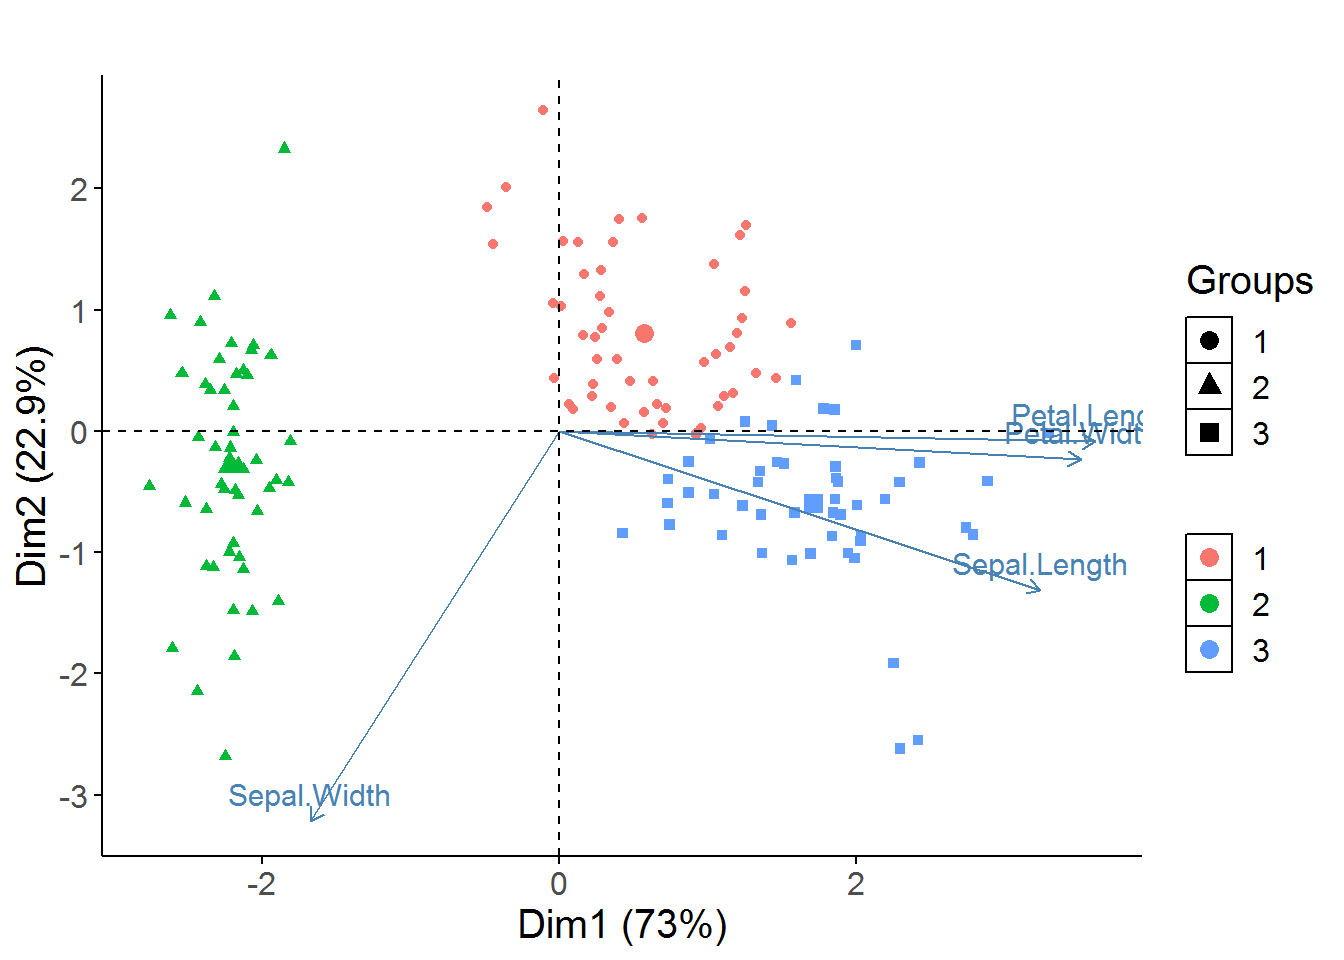
\includegraphics{Taller3_files/figure-latex/unnamed-chunk-11-1.pdf}

\begin{Shaded}
\begin{Highlighting}[]
\KeywordTok{ggplot}\NormalTok{(}\DataTypeTok{data=}\NormalTok{Reflectancia, }\KeywordTok{aes}\NormalTok{(Species,D_720nm)) }\OperatorTok{+}\StringTok{ }\KeywordTok{geom_boxplot}\NormalTok{() }\OperatorTok{+}\StringTok{ }\KeywordTok{ggtitle}\NormalTok{(}\StringTok{"Comportamiento Firma 720 nm"}\NormalTok{) }\OperatorTok{+}\StringTok{ }\KeywordTok{xlab}\NormalTok{(}\StringTok{"Especies"}\NormalTok{) }\OperatorTok{+}\StringTok{ }\KeywordTok{ylab}\NormalTok{(}\StringTok{"Reflectancia"}\NormalTok{)}
\end{Highlighting}
\end{Shaded}

\includegraphics{Taller3_files/figure-latex/unnamed-chunk-11-2.pdf}

\begin{Shaded}
\begin{Highlighting}[]
\CommentTok{# Prueba de Dixon}

\KeywordTok{dixon.test}\NormalTok{(}\KeywordTok{sample}\NormalTok{(Reflectancia}\OperatorTok{$}\NormalTok{D_560nm, }\DataTypeTok{size=}\DecValTok{30}\NormalTok{))}
\end{Highlighting}
\end{Shaded}

\begin{verbatim}
## 
##  Dixon test for outliers
## 
## data:  sample(Reflectancia$D_560nm, size = 30)
## Q = 0.20418, p-value = 0.8265
## alternative hypothesis: highest value 44.74 is an outlier
\end{verbatim}

\begin{Shaded}
\begin{Highlighting}[]
\KeywordTok{dixon.test}\NormalTok{(}\KeywordTok{sample}\NormalTok{(Reflectancia}\OperatorTok{$}\NormalTok{D_720nm, }\DataTypeTok{size=}\DecValTok{30}\NormalTok{))}
\end{Highlighting}
\end{Shaded}

\begin{verbatim}
## 
##  Dixon test for outliers
## 
## data:  sample(Reflectancia$D_720nm, size = 30)
## Q = 0.18756, p-value = 0.9448
## alternative hypothesis: highest value 78.57 is an outlier
\end{verbatim}

Viendo que para la longitud de onda de 560 no existen valores atípicos
mientrás que para el de 720 nm si para la especie SS.

\hypertarget{punto-9-outliers-multivariados}{%
\section{Punto 9: Outliers
multivariados}\label{punto-9-outliers-multivariados}}

Para observar los valores atípicos multivariados es realizado a partir
del estadístico T\(^2\) y comparado con el percentil que este posee con
la distribución chi cuadrado.

\begin{Shaded}
\begin{Highlighting}[]
\NormalTok{vec.medias=}\KeywordTok{apply}\NormalTok{(Reflectancia[,}\DecValTok{1}\OperatorTok{:}\DecValTok{2}\NormalTok{],}\DecValTok{2}\NormalTok{,mean);vec.medias}
\end{Highlighting}
\end{Shaded}

\begin{verbatim}
##  D_560nm  D_720nm 
## 14.30139 35.78806
\end{verbatim}

\begin{Shaded}
\begin{Highlighting}[]
\NormalTok{T2=}\KeywordTok{c}\NormalTok{()}
\ControlFlowTok{for}\NormalTok{(j }\ControlFlowTok{in} \DecValTok{1}\OperatorTok{:}\KeywordTok{dim}\NormalTok{(Reflectancia)[}\DecValTok{1}\NormalTok{])\{}
\NormalTok{  T2[j]=}\KeywordTok{c}\NormalTok{((}\KeywordTok{t}\NormalTok{(}\KeywordTok{t}\NormalTok{(Reflectancia[j,}\DecValTok{1}\OperatorTok{:}\DecValTok{2}\NormalTok{])}\OperatorTok{-}\NormalTok{(vec.medias)))}\OperatorTok\KeywordTok{solve}\NormalTok{(}\KeywordTok{var}\NormalTok{(Reflectancia[,}\DecValTok{1}\OperatorTok{:}\DecValTok{2}\NormalTok{]))}\OperatorTok\KeywordTok{as.matrix}\NormalTok{(}\KeywordTok{t}\NormalTok{(Reflectancia[j,}\DecValTok{1}\OperatorTok{:}\DecValTok{2}\NormalTok{])}\OperatorTok{-}\NormalTok{(vec.medias)))}
\NormalTok{\}}
\NormalTok{T2}
\end{Highlighting}
\end{Shaded}

\begin{verbatim}
##  [1]  1.26541020  1.09383567  1.24128875  1.67375718  0.45417223  0.41656430
##  [7]  0.27561128  0.34847917  0.04318851  0.07844282  0.10339451 12.43210949
## [13]  0.05790637  0.13704612  0.07555811  0.05807567  0.09033585  0.25119830
## [19]  0.47601009  0.19901130  7.16415107 10.42111846  5.77865326 11.83215879
## [25]  0.57530618  0.82479717  0.68473177  0.71821599  0.39872455  0.69415980
## [31]  0.40375328  0.53175909  0.88021407  0.12249645  0.14489054  8.05347359
\end{verbatim}

\begin{Shaded}
\begin{Highlighting}[]
\NormalTok{LS=}\KeywordTok{qchisq}\NormalTok{(}\FloatTok{0.95}\NormalTok{,}\DataTypeTok{df=}\KeywordTok{dim}\NormalTok{(Reflectancia)}\OperatorTok{-}\DecValTok{1}\NormalTok{)}
\NormalTok{colores=}\KeywordTok{ifelse}\NormalTok{(T2}\OperatorTok{>}\NormalTok{LS,}\StringTok{"darkred"}\NormalTok{,}\StringTok{"darkgreen"}\NormalTok{)}
\KeywordTok{plot}\NormalTok{(T2,}\DataTypeTok{col=}\NormalTok{colores,}\DataTypeTok{pch=}\DecValTok{19}\NormalTok{,}\DataTypeTok{cex=}\FloatTok{0.85}\NormalTok{,}\DataTypeTok{xlab=}\StringTok{"Observación")}
\StringTok{grid(20,20,col="}\NormalTok{lightblue}\StringTok{")}
\StringTok{abline(h=LS)}
\StringTok{etiquetas=which(T2>LS)}
\StringTok{text(etiquetas,c(LS)+0.4,"}\NormalTok{outlier}\StringTok{")}
\end{Highlighting}
\end{Shaded}

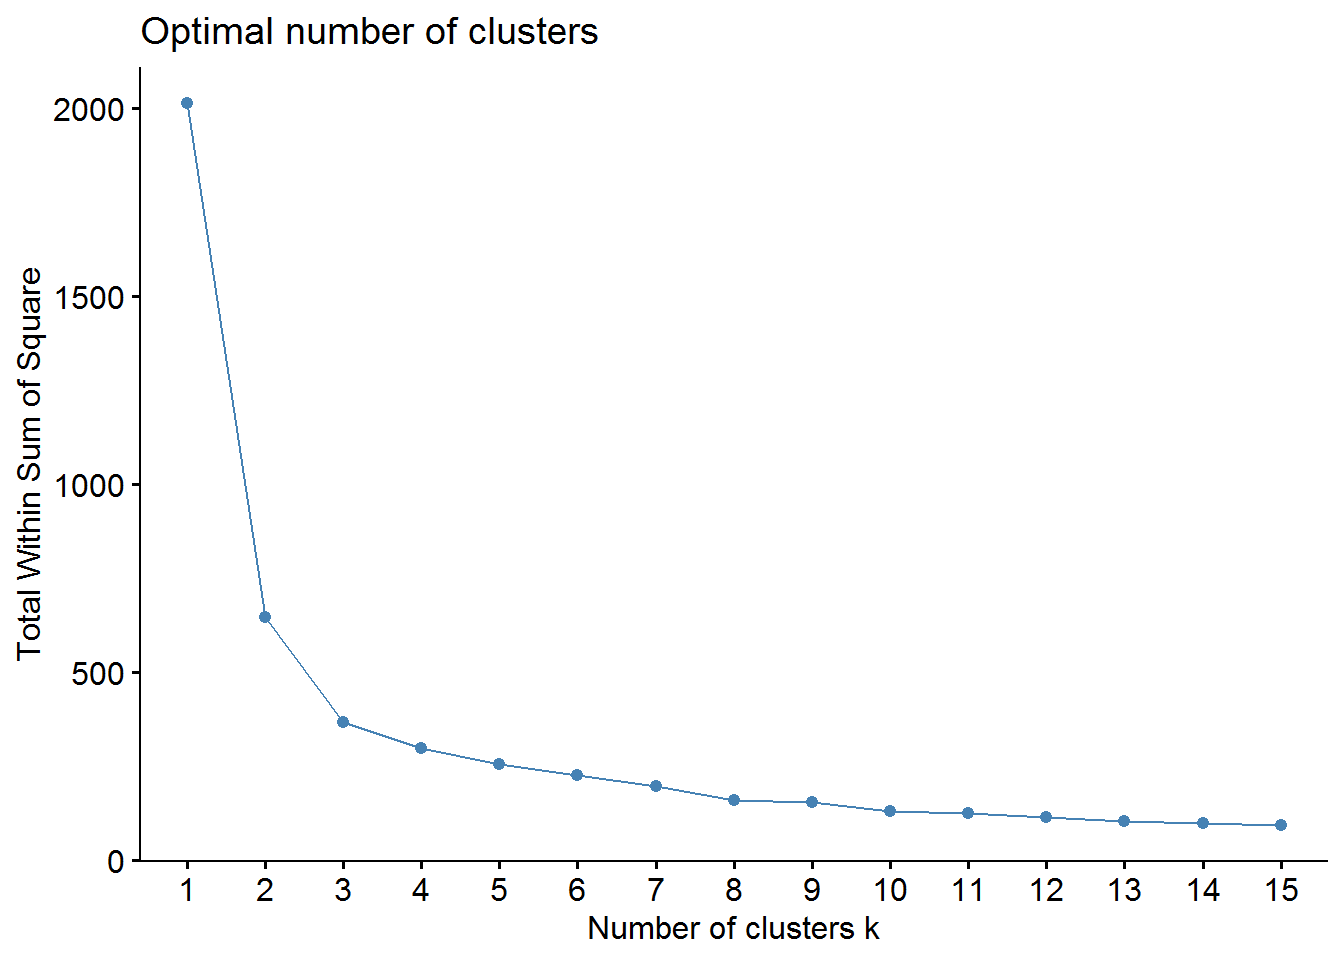
\includegraphics{Taller3_files/figure-latex/unnamed-chunk-12-1.pdf}

\begin{Shaded}
\begin{Highlighting}[]
\KeywordTok{plot}\NormalTok{(Reflectancia}\OperatorTok{$}\NormalTok{D_560nm,Reflectancia}\OperatorTok{$}\NormalTok{D_720nm,}\DataTypeTok{pch=}\DecValTok{19}\NormalTok{,}\DataTypeTok{col=}\NormalTok{colores)}
\KeywordTok{grid}\NormalTok{(}\DecValTok{20}\NormalTok{,}\DecValTok{20}\NormalTok{,}\DataTypeTok{col=}\StringTok{"lightblue"}\NormalTok{)}
\end{Highlighting}
\end{Shaded}

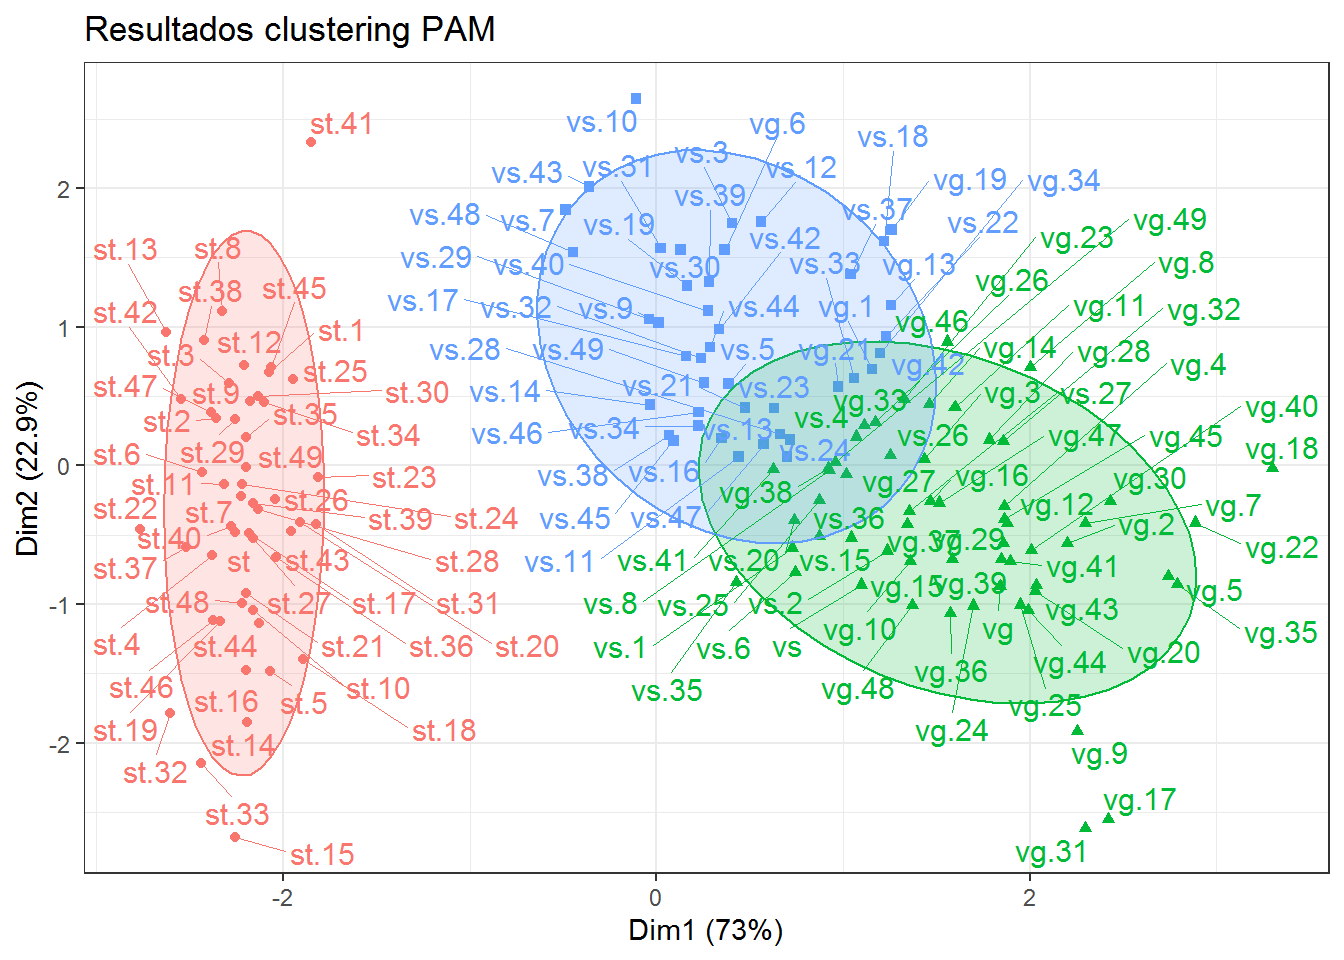
\includegraphics{Taller3_files/figure-latex/unnamed-chunk-12-2.pdf}

Lo anterior arrojo como resultado que los datos poseen 4 datos
multivariados.

\hypertarget{punto-10-comparaciuxf3n-de-medias-por-cada-respuesta}{%
\section{Punto 10: Comparación de medias por cada
respuesta}\label{punto-10-comparaciuxf3n-de-medias-por-cada-respuesta}}

\end{document}
